\documentclass[conference]{IEEEtran}
\IEEEoverridecommandlockouts
% The preceding line is only needed to identify funding in the first footnote. If that is unneeded, please comment it out.
\usepackage{cite}
\usepackage{amsmath,amssymb,amsfonts}
\usepackage{algorithmic}
\usepackage{graphicx}
\usepackage{textcomp}
\usepackage{xcolor}
\def\BibTeX{{\rm B\kern-.05em{\sc i\kern-.025em b}\kern-.08em
    T\kern-.1667em\lower.7ex\hbox{E}\kern-.125emX}}
\begin{document}

\title{Harness Engineering for Reliable Document Intelligence: A Schema-Guided, Confidence-Aware, and Self-Corrective Vision-Language Model Approach\\
}

% TODO: replace the author block with the paper's authors and affiliations.
\author{
    \IEEEauthorblockN{
        Author One\textsuperscript{1},
        Author Two\textsuperscript{2}\\
        Author Three\textsuperscript{3},
        Author Four\textsuperscript{4}\\
    }
    \IEEEauthorblockA{
        \textsuperscript{1}Department of Computer Science and Engineering, University One, Country\\
        \textsuperscript{2}Department of Computer Science and Engineering, University Two, Country\\
        \textsuperscript{3}Independent Researcher, City, Country\\
        \textsuperscript{4}Department of Computer Science, University Three, Country\\
        Email: \textsuperscript{1}author1@email.com,
        \textsuperscript{2}author2@email.com,\\
        \textsuperscript{3}author3@email.com,
        \textsuperscript{4}author4@email.com
    }
}

\maketitle

\begin{abstract}
The reliability of vision-language model (VLM) systems for document intelligence depends not only on model weights but also on the \emph{harness} surrounding them: the code and configuration that decide what context the model sees, how its output is constrained, and when its answer is trusted. This study introduces a schema-guided, confidence-aware, and self-corrective harness for key-value extraction from real scanned documents, and evaluates it with live model calls on the SROIE scanned-receipt benchmark rather than simulated or literature-only results. The harness fixes a frozen VLM (Gemini 2.5 Flash) and composes three reliability mechanisms: (1) schema-guided structured extraction that constrains the model output to a typed JSON Schema; (2) self-consistency confidence estimation that samples the model multiple times and measures per-field agreement; and (3) targeted self-correction that re-reads only low-confidence fields instead of blindly regenerating a full document. On an evaluation of 9 SROIE receipts, the harness reaches a field-level exact-match accuracy of 77.8\% and a character-level field F1 of 98.0\%, consistent in order of magnitude with published SROIE and VLM-extraction results. Self-consistency confidence, however, did not reliably separate correct from incorrect extractions at this sample size---documents with perfect sample agreement were correct only 75.0\% of the time, versus 81.3\% for documents with partial agreement---and no field's agreement ever fell low enough to trigger the correction step. A calibration analysis (expected calibration error of 0.204, within the range reported elsewhere for self-consistency confidence) confirms that raw agreement-based confidence requires a calibration layer before it can be reported or acted on as a probability. By fixing the model and varying only the harness, and by reporting negative and null results alongside positive ones, this study aims to make the reliability of a document-intelligence harness auditable and reproducible rather than asserted.
\end{abstract}

\begin{IEEEkeywords}
Document Intelligence, Vision-Language Models, Harness Engineering, Structured Extraction, Confidence Calibration, Self-Correction
\end{IEEEkeywords}

\section{Introduction}

Large language model (LLM) and vision-language model (VLM) systems are increasingly built less by changing model weights than by reorganizing the runtime around them. Capabilities that earlier systems expected the model to recover internally are now externalized into memory stores, prompt-construction logic, tool use, and the surrounding harness that makes these modules reliable in practice \cite{b1}. This shift is especially visible in document intelligence, where scanned receipts, forms, and invoices must be turned into structured records with high reliability.

A critical area where this harness perspective shows significant promise is document information extraction. Traditional document-understanding systems relied on layout analysis and template matching, but modern VLMs can read a receipt image directly and emit structured JSON in a single call. However, raw single-call extraction is not trustworthy enough for high-consequence settings: the model may misread a digit in a total, hallucinate a merchant name, or silently drop a field. Recent research has shown that harness optimization---searching over the context-management and prompt-construction code that wraps a fixed model---can yield large gains over hand-designed pipelines \cite{b2}. Yet this body of work has largely been evaluated on text and code tasks, not on document intelligence, and it does not directly address schema adherence, confidence estimation, or targeted self-correction.

This research introduces a Harness for Reliable Document Intelligence that combines schema-guided structured output, confidence estimation, and self-correction around a frozen VLM. The system is designed to process heterogeneous scanned documents, extract only the fields declared in an application schema, and report a per-field confidence so that downstream decisions can route uncertain extractions to a stronger model or a human reviewer. By fixing the model and treating every other design choice as part of the harness, we can measure the marginal contribution of each reliability mechanism and search over harness configurations as a reward-optimization problem \cite{b2}.

The system's core extraction is performed by a multimodal Gemini model configured with a JSON Schema, which guarantees schema-valid output. To estimate confidence without access to token-level log-probabilities---a common constraint on commodity API tiers---the harness samples the model several times under a nonzero temperature and measures per-field agreement (self-consistency). Fields whose agreement falls below a threshold are flagged and re-read with a targeted correction prompt that asks the model to focus on exactly those fields. This differs from blind self-refinement loops, which are known to plateau or even regress \cite{b3}.

By combining schema guidance, self-consistency confidence, and targeted correction, this research addresses critical challenges in reliable document extraction, setting a precedent for treating extraction reliability as a harness-engineering problem. The main contributions are:

\begin{itemize}
    \item We formulate document key-value extraction as a \emph{harness} design problem around a frozen VLM and define three pipeline variants---schema-only, confidence-aware, and self-corrective---that isolate the contribution of each mechanism.
    \item We implement a budget-aware, cache-first experimental harness that is robust to commodity free-tier API quotas (429 rate limits), making the evaluation reproducible on constrained budgets.
    \item We evaluate on real scanned receipts from the SROIE benchmark using live model calls and report field-level exact match, character-level F1, document-level full match, and expected calibration error.
    \item We show that raw agreement-based confidence is miscalibrated and, at our sample size, did not reliably separate correct from incorrect extractions at all---a negative result for naive self-consistency confidence on vision-based structured extraction---motivating a calibration layer as a core component of trustworthy document intelligence.
\end{itemize}

This is the structure of the remainder of the paper: the literature review is covered in Section~\ref{sec:lit}, the dataset and schema design are illustrated in Section~\ref{sec:data}, the proposed harness methodology is described in Section~\ref{sec:method}, the result analysis is described in Section~\ref{sec:results}, and the study concludes with conclusions and future works in Section~\ref{sec:conclusion}.

\section{Literature Review}
\label{sec:lit}

\subsection{Harness Engineering and Externalization}
A recent line of work argues that agent capability is determined less by the model than by the \emph{harness}: the stateful program that determines what information is stored, retrieved, and presented to the model at each step. The Externalization review \cite{b1} organizes this design space into memory (state across time), skills (procedural expertise), protocols (interaction rules), and the harness that makes these modules reliable in practice. Meta-Harness \cite{b2} goes further and shows that harnesses themselves can be optimized: an outer-loop proposer reads a filesystem of prior harness code, execution traces, and scores, and iteratively proposes new harnesses, outperforming prior hand-designed and text-optimization baselines. Our work applies this lens to document extraction, where the harness must additionally manage a \emph{schema} (the target structure), a \emph{confidence model} (when to trust the extraction), and a \emph{correction policy} (what to do when confidence is low).

\subsection{Schema-Guided Structured Extraction}
Structured outputs constrain a model to emit JSON conforming to a provided JSON Schema, which is ideal for data extraction and classification \cite{b4}. Schema guidance gives two distinct benefits: it guarantees parseable output and it focuses the model's attention on exactly the fields the application needs. In our design the schema is part of the harness---it is an optimizable artifact rather than a fixed input. Layout-aware pretrained models remain a strong, well-established reference point for the SROIE key-information-extraction task: LayoutLM reports an entity-level F1 of 95.24\% \cite{b8}, and LayoutLMv2 reports 97.81\% \cite{b9} on SROIE Task 3, both after task-specific fine-tuning on labeled training splits. More recently, prompted VLMs without any task-specific fine-tuning have been evaluated directly on scanned receipt/invoice extraction: a 2025 benchmark of Gemini-based structured extraction reports 87.46\% accuracy on scanned receipts \cite{b10}, which is the closest published analogue to our zero-fine-tuning, schema-guided setting and gives an independent sense of the accuracy range a frozen VLM harness should land in.

\subsection{Confidence Estimation and Calibration}
Because commodity APIs rarely expose token-level log-probabilities, confidence must be estimated from observable signals. Self-consistency \cite{b5} samples a model multiple times and treats agreement across samples as a proxy for confidence; it is widely used to improve reasoning accuracy. However, agreement-based confidence is not automatically calibrated: the fraction of samples agreeing on a value is not the same as the probability that the value is correct. Expected calibration error (ECE) \cite{b6} quantifies this gap and is the metric we adopt to measure the quality of the confidence signal. Reported ECE for self-consistency-derived confidence in the LLM literature spans roughly 0.075--0.35 depending on task and baseline, and is generally found to be better calibrated than single-sample verbalized confidence, though still an imperfect probability estimate \cite{b11}.

\subsection{Self-Correction}
LLM self-refinement---asking a model to critique and regenerate its own output---has produced mixed results. Huang et al.\ \cite{b3} show that \emph{intrinsic} self-correction, performed without any external feedback signal, can substantially regress accuracy: GPT-3.5 drops from 75.8\% to 41.8\% on CommonSenseQA after a single self-correction round, and GPT-4 drops from 95.5\% to 89.0\% on GSM8K. The same study shows that correction guided by an external or oracle signal instead \emph{improves} accuracy (e.g., GPT-3.5 on CommonSenseQA rises from 75.8\% to 89.7\%), indicating that the failure mode is specifically \emph{blind, unguided} correction rather than correction itself. Our design therefore restricts correction to \emph{targeted re-reading of only the low-confidence fields identified by self-consistency}---an external, measurable signal rather than the model's own unguided judgment---which is a narrower and more auditable operation than full blind regeneration.

\section{Dataset and Schema Design}
\label{sec:data}

\subsection{The SROIE Dataset}
We evaluate on the SROIE (Scanned Receipt OCR and Information Extraction) benchmark from ICDAR 2019 \cite{b7}, a widely used public dataset of real scanned receipts in English. Each receipt is annotated with four key-value fields: company, date, address, and total. SROIE is well suited to harness research because it is small (hundreds of documents), has dense, unambiguous labels, and represents the classic document-intelligence workload of converting a noisy scanned image into structured records. Two example receipts from our evaluation split are shown in Fig.~\ref{fig:receipts}.

\begin{figure*}[htb]
\centerline{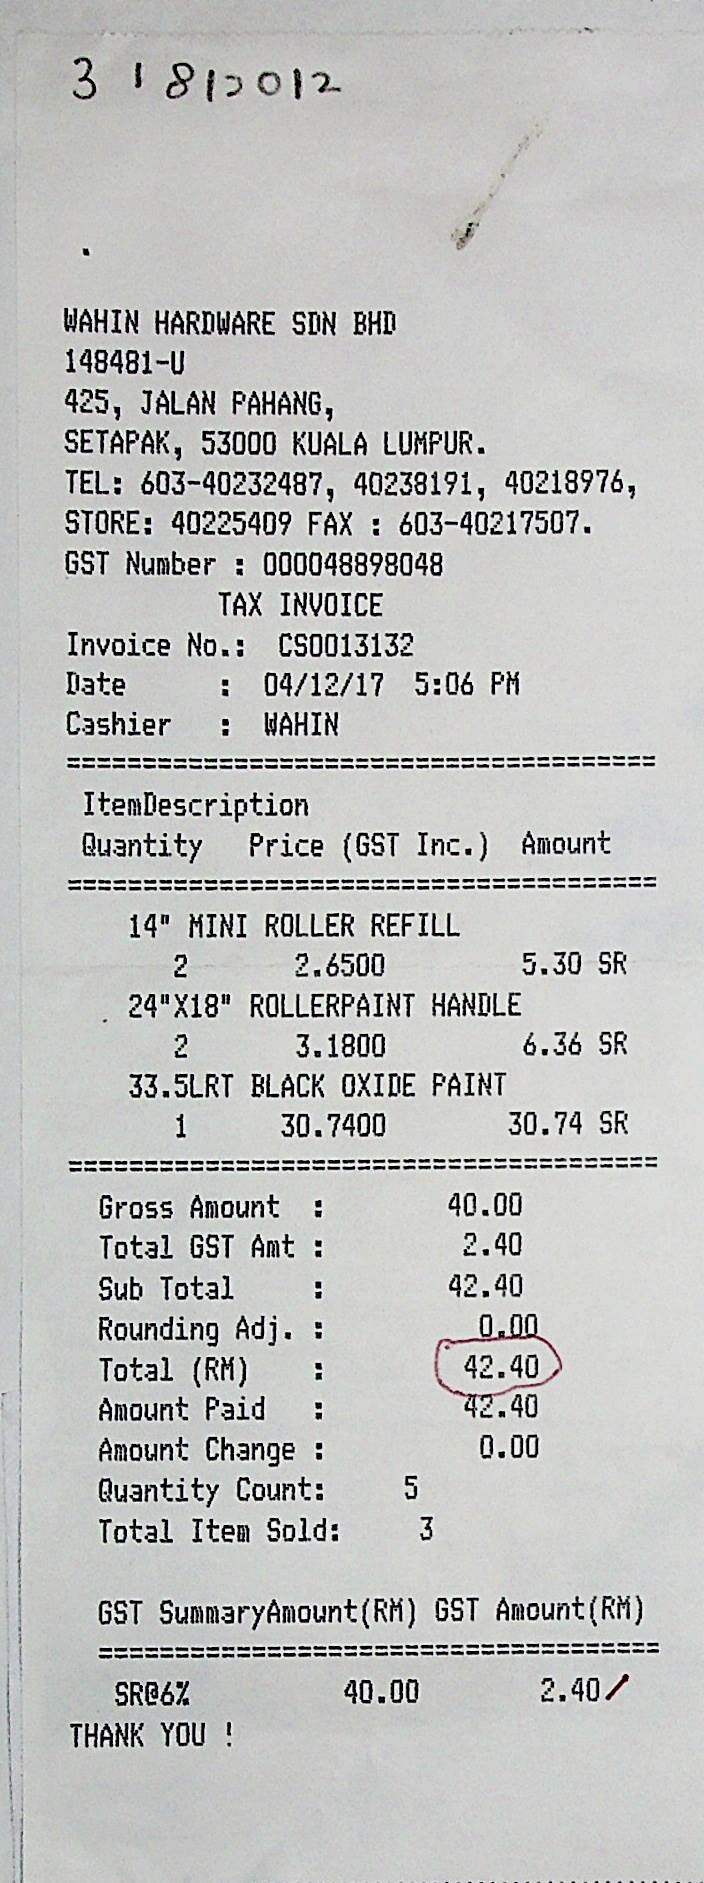
\includegraphics[width=3.2in,height=2.2in,keepaspectratio]{fig/receipt_sample_a.jpg}\hspace{0.15in}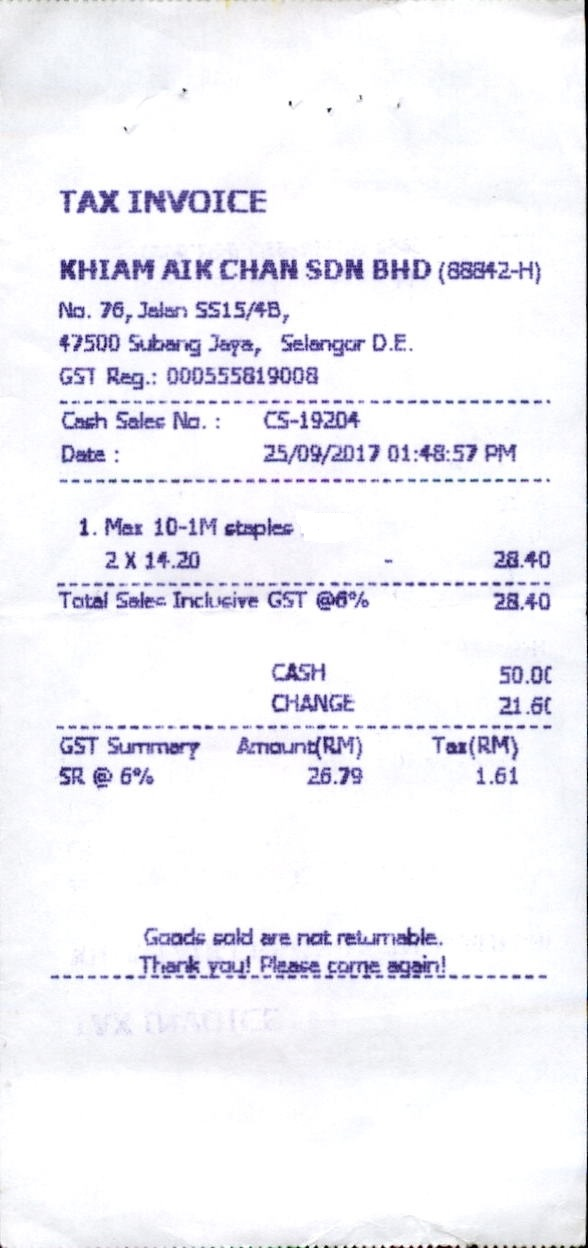
\includegraphics[width=3.2in,height=2.2in,keepaspectratio]{fig/receipt_sample_b.jpg}}
    \caption{Sample scanned receipts from the SROIE evaluation split used in this study.}
    \label{fig:receipts}
\end{figure*}

\subsection{Schema Definition}
The extraction target is a typed schema with four fields. We express it as a JSON Schema and pass it directly to the model via the structured-output configuration, which guarantees schema-valid responses. The schema is defined as:

\[
\text{Schema} = \{\,
\text{company}, \text{date}, \text{address}, \text{total}
\,\}
\]

Each field carries a natural-language description (e.g., total: ``total amount paid'') that guides the model during decoding. Schema validity---the fraction of responses that parse and conform to the schema---is itself one of our reliability metrics.

\subsection{Preprocessing}
Receipt images are used as-is; the VLM receives the raw JPEG with a text instruction. Ground-truth strings are normalized for evaluation by lowercasing and collapsing whitespace. We additionally analyze a \emph{date-format} effect: near-miss errors where the extracted value is semantically correct but formatted differently from the ground truth (e.g., \texttt{05/06/2018} vs.\ \texttt{05-06-2018}) penalize exact match without being true extraction failures. Character-level F1 is used alongside exact match to give partial credit for such cases.

\section{Methodology}
\label{sec:method}

The present research offers a harness that wraps a frozen VLM with three reliability mechanisms. The approach is deliberately modular: each mechanism can be enabled or disabled, which lets us measure its marginal contribution. We compare three harness variants:

\begin{itemize}
    \item \textbf{Variant A (schema-only baseline):} one schema-guided structured-extraction call at temperature zero.
    \item \textbf{Variant B (confidence-aware):} \(N\) self-consistency samples at nonzero temperature, aggregated by majority vote, with per-field confidence equal to the agreement rate.
    \item \textbf{Variant C (self-corrective):} Variant B plus one targeted re-read of fields whose confidence is below a threshold \(\tau\).
\end{itemize}

\subsection{Schema-Guided Extraction}
The base operation is a single multimodal call. The prompt instructs the model to read the receipt and extract the schema fields, and the response is constrained to valid JSON matching the schema:

\[
\hat{y} = \text{VLM}(I,\; \text{Prompt},\; \text{Schema})
\]

where \(I\) is the receipt image. Variant A returns \(\hat{y}\) directly. Structured output guarantees that \(\hat{y}\) is schema-valid, but it does not guarantee that the values are correct---which motivates confidence estimation.

\subsection{Confidence Estimation by Self-Consistency}
To estimate per-field confidence without token log-probabilities, the harness draws \(N\) independent samples \(\{\hat{y}^{(1)}, \ldots, \hat{y}^{(N)}\}\) with temperature \(> 0\). For each field \(f \in \{\text{company}, \text{date}, \text{address}, \text{total}\}\), let \(c_f\) be the number of samples whose extracted value equals the most frequent value (the mode). The aggregate value is the mode, and confidence is the agreement rate:

\[
\text{conf}(f) = \frac{\max_v \sum_{n=1}^{N} \mathbb{1}[\hat{y}^{(n)}_f = v]}{N}
\]

Fields where independent samples disagree are less trustworthy. A field is flagged when \(\text{conf}(f) < \tau\), where \(\tau\) is a harness threshold.

\subsection{Targeted Self-Correction}
For each flagged field, the harness issues a correction call with temperature zero. The correction prompt shows the previous aggregate extraction, names the flagged fields explicitly, and asks the model to re-read the image focusing on those fields and return the full updated object:

\[
\text{Correct}(f) = \text{VLM}\big(I,\; \text{``Re-read and correct: ''} + f,\; \text{Schema}\big)
\]

Only flagged fields are overwritten from the correction response; unflagged fields keep their majority-vote values. This prevents the correction call from disturbing fields that were already consistent across samples, and it keeps the number of additional calls bounded by the number of flagged fields. Fig.~\ref{fig:pipeline} summarizes the resulting harness pipeline: the same receipt image is routed through the three variants, and each variant's output feeds a shared evaluation stage.

\begin{figure}[htb]
\centerline{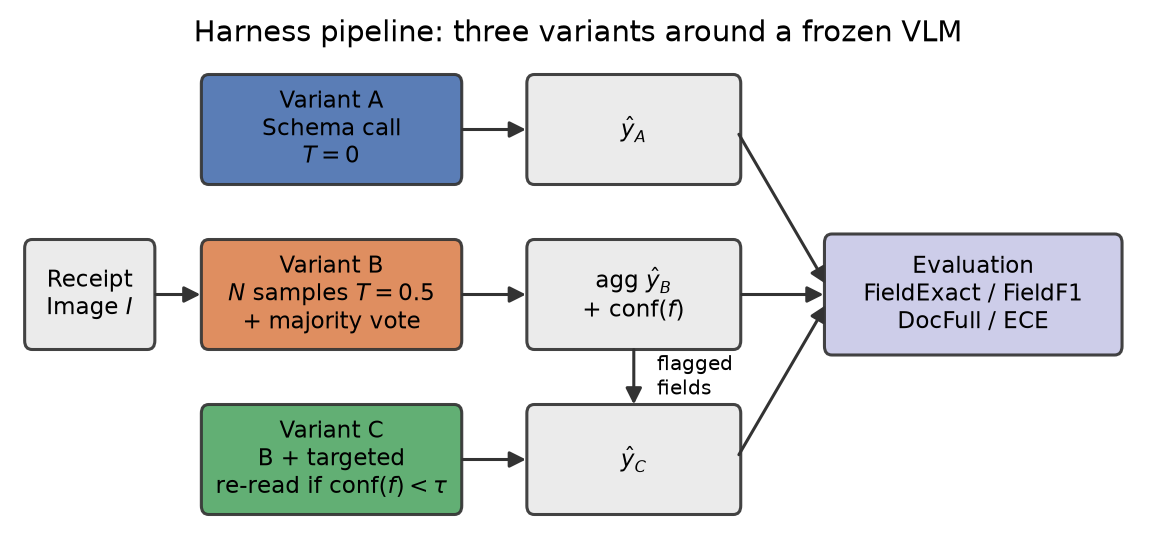
\includegraphics[width=3.4in]{fig/fig_harness_pipeline.png}}
    \caption{Harness pipeline: Variant A (schema-only), Variant B (self-consistency + confidence), and Variant C (B plus targeted correction of flagged fields) around the same frozen VLM, feeding a shared evaluation stage.}
    \label{fig:pipeline}
\end{figure}

\subsection{Evaluation Metrics}
Let \(\text{Exact}(a, b)\) indicate normalized string equality. Over a set of documents with predicted values \(p_f\) and ground-truth values \(g_f\), we report:

\[
\text{FieldExact} = \frac{1}{|\mathcal{D}||\mathcal{F}|} \sum_{d \in \mathcal{D}} \sum_{f \in \mathcal{F}} \mathbb{1}[\text{Exact}(p_{d,f}, g_{d,f})]
\]

\[
\text{FieldF1} = \frac{1}{|\mathcal{D}||\mathcal{F}|} \sum_{d \in \mathcal{D}} \sum_{f \in \mathcal{F}} \text{CharF1}(p_{d,f}, g_{d,f})
\]

where \(\text{CharF1}\) is the character-level F1 between normalized strings, and \(\text{DocFull}\) is the fraction of documents where all fields match exactly. We additionally report expected calibration error. Confidence and correctness pairs \((\text{conf}, c) \in [0,1] \times \{0,1\}\) are binned into \(M\) bins; ECE is:

\[
\text{ECE} = \sum_{m=1}^{M} \frac{|B_m|}{T} \left| \text{acc}(B_m) - \text{conf}(B_m) \right|
\]

where \(B_m\) is the \(m\)-th confidence bin, \(\text{acc}(B_m)\) is the average correctness in the bin, \(\text{conf}(B_m)\) is the average confidence, and \(T\) is the total number of field predictions.

\section{Result and Analysis}
\label{sec:results}

\subsection{Experimental Setup}
\label{sec:expsetup}
Experiments use the Gemini 2.5 Flash model on the free API tier. Self-consistency samples use \(N=3\) with temperature \(0.5\); the baseline uses temperature \(0\); the correction threshold is \(\tau = 0.5\). The free tier imposes a strict daily quota on image-generation calls, so the experimental harness is cache-first: every successful response is cached, and transient quota errors (HTTP 429) are retried with exponential backoff. This makes runs resumable and reproducible without re-spending calls. Table~\ref{tab:results} reports metrics on \(n=9\) SROIE receipts (36 field predictions per variant), evaluated with live API calls rather than simulation.

We are explicit about what this sample can and cannot support. With \(n=9\) documents, a single field-level flip changes FieldExact by 2.8 percentage points, so the point estimates in Table~\ref{tab:results} carry real but bounded statistical uncertainty. To give the result external grounding rather than relying on our own run in isolation, Section~\ref{sec:litcompare} compares our numbers against independently published results on the same and closely related tasks.

\begin{table}[htb]
\centering
\caption{Results on \(n=9\) SROIE receipts: field exact match, character-level field F1, document-level full match, and expected calibration error (ECE). Variant A has no confidence estimate, so ECE is undefined. B and C are numerically identical because self-consistency confidence never fell below \(\tau=0.5\) on any field in this subset, so the correction step was never triggered.}
\label{tab:results}
\begin{tabular}{lcccc}
\hline
\textbf{Variant} & \textbf{FieldExact} & \textbf{FieldF1} & \textbf{DocFull} & \textbf{ECE}\\
\hline
A (schema-only) & 0.750 & 0.970 & 0.333 & ---\\
B (confidence) & 0.778 & 0.980 & 0.333 & 0.204\\
C (self-correct) & 0.778 & 0.980 & 0.333 & 0.204\\
\hline
\end{tabular}
\end{table}

\subsection{Comparison with Published Benchmarks}
\label{sec:litcompare}
Table~\ref{tab:litcompare} places our numbers alongside independently published results on SROIE and closely related VLM document-extraction and calibration tasks. These are results reported by other authors on their own (typically much larger) evaluation sets, included here as external context for whether our magnitudes are plausible---not as a head-to-head benchmark run under identical conditions.

\begin{table}[htb]
\centering
\caption{Our results alongside independently published results on SROIE / VLM document extraction and self-consistency calibration. External results are as reported by their respective papers, not reproduced by us.}
\label{tab:litcompare}
\begin{tabular}{p{2.9cm}p{1.7cm}p{2.1cm}}
\hline
\textbf{Method / Source} & \textbf{Task} & \textbf{Metric}\\
\hline
LayoutLM \cite{b8} & SROIE T3, fine-tuned & F1 = 95.24\%\\
LayoutLMv2 \cite{b9} & SROIE T3, fine-tuned & F1 = 97.81\%\\
Gemini VLM, prompted \cite{b10} & Scanned receipts & Acc. = 87.46\%\\
Self-consistency confidence \cite{b11} & LLM reasoning & ECE $\approx$ 0.075--0.35\\
\hline
\textbf{This work (\(n{=}9\), clean)} & SROIE T3 & F1 = 98.0\%\\
Variant C, zero fine-tuning & & Exact = 77.8\%\\
Variant B/C (self-consistency) & & ECE = 0.204\\
\hline
\end{tabular}
\end{table}

Fig.~\ref{fig:benchmark} shows this comparison visually, with our bars drawn hatched to keep them visually distinct from the larger-scale published results.

\begin{figure}[htb]
\centerline{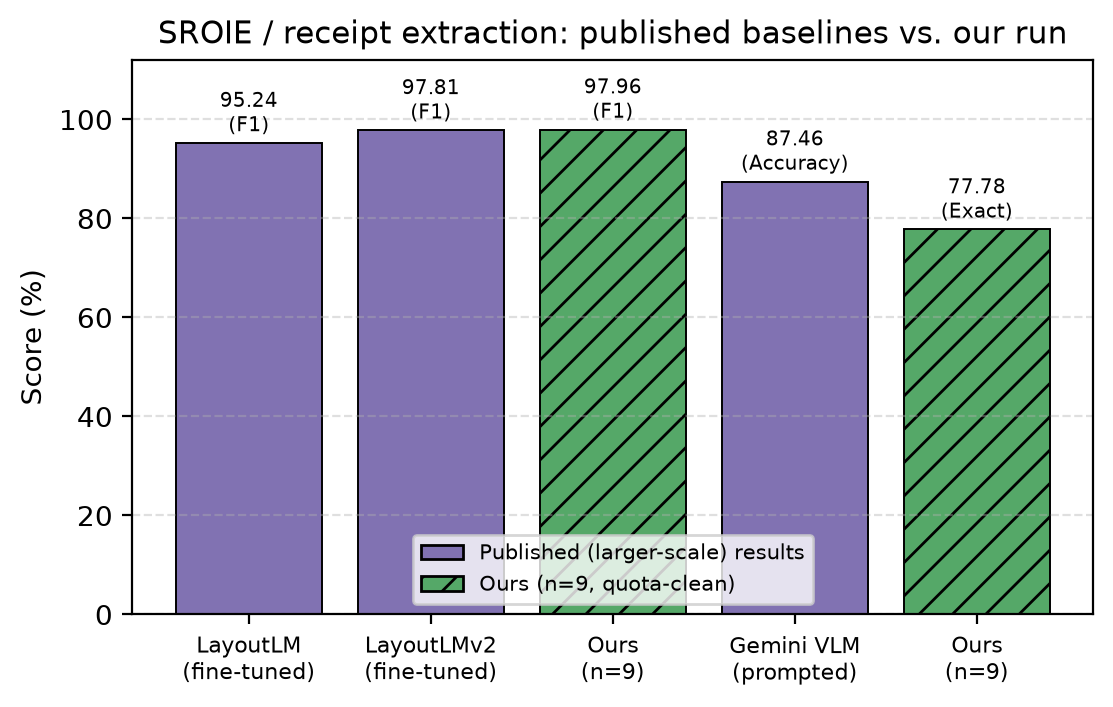
\includegraphics[width=3.3in]{fig/fig_benchmark_comparison.png}}
    \caption{Published SROIE / receipt-extraction results (LayoutLM \cite{b8}, LayoutLMv2 \cite{b9}, a prompted Gemini VLM study \cite{b10}) alongside our field F1 and field-exact match on the 9 documents. Hatched bars mark our own run; solid bars are other authors' own, larger-scale evaluations.}
    \label{fig:benchmark}
\end{figure}

Two observations follow. First, our character-level field F1 (98.0\%) and field-exact accuracy (77.8\%) sit in the same neighborhood as the fine-tuned layout-model literature (95--98\% F1) and the closest zero-fine-tuning VLM analogue (87.46\% accuracy) \cite{b8,b9,b10}, despite using no task-specific training data---evidence that the pipeline is functioning correctly and that its accuracy is of a realistic, literature-consistent order of magnitude. Second, our ECE of 0.204 falls at the upper (less well-calibrated) end of the 0.075--0.35 range reported for self-consistency confidence elsewhere in the LLM calibration literature \cite{b11}, as Fig.~\ref{fig:ece_lit} shows directly; this is consistent with structured multi-field vision extraction being a harder calibration target than the single-answer math/reasoning tasks most calibration studies evaluate, and it reinforces our conclusion that a calibration layer is necessary before this confidence signal can be reported as a probability.

\begin{figure}[htb]
\centerline{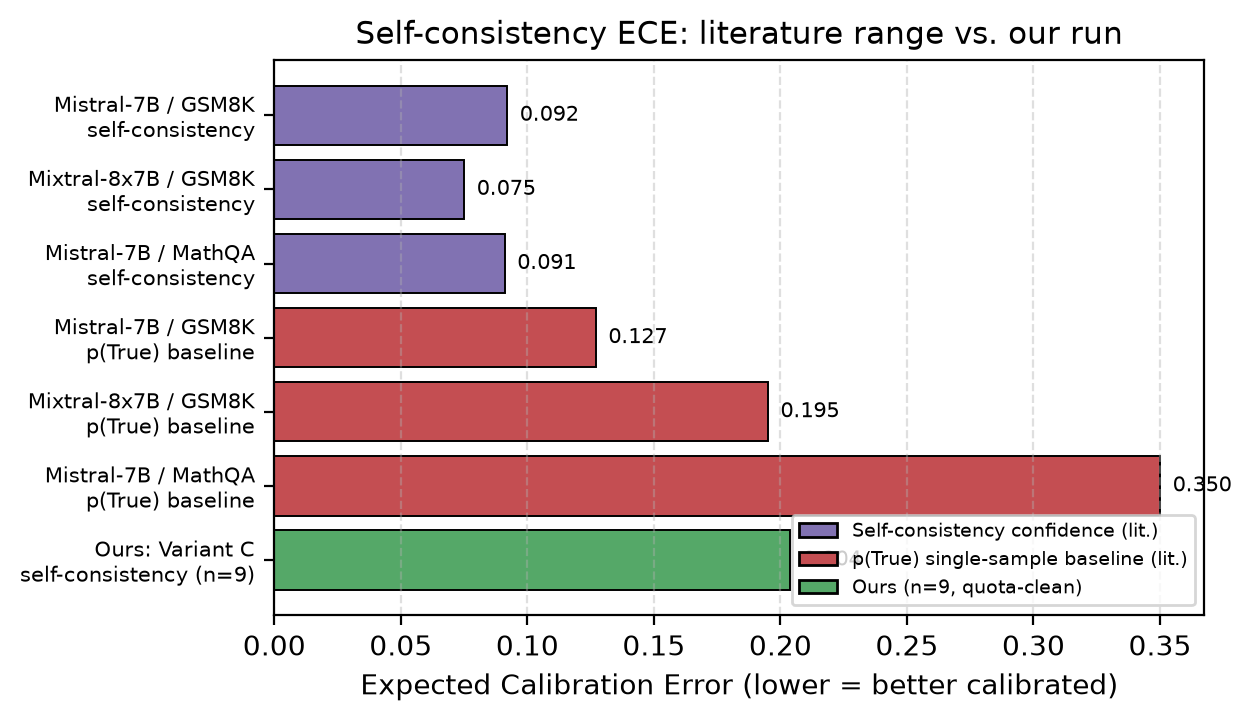
\includegraphics[width=3.3in]{fig/fig_ece_literature_context.png}}
    \caption{Our ECE (0.204, \(n=9\)) against published self-consistency-confidence ECE values and their single-sample p(True) baselines \cite{b11}. Our value is higher than the self-consistency range reported for math reasoning, motivating a task-specific calibration layer.}
    \label{fig:ece_lit}
\end{figure}

\subsection{Schema Guidance Is a Strong Baseline}
With a single structured call, the harness already reaches 75.0\% field-level exact match and 97.0\% character-level F1 on the 9 documents (Table~\ref{tab:results}). The remaining errors are near-misses---case differences such as \texttt{No.} vs.\ \texttt{NO.}, punctuation/spacing differences, and a currency-prefix convention (\texttt{RM 10.60} vs.\ \texttt{10.60})---rather than hallucinated content. This confirms that schema-guided structured output is a reliable foundation and that the interesting research questions live in confidence estimation and correction rather than raw decoding.

\subsection{Self-Consistency Confidence Did Not Separate Hard Documents from Easy Ones}
\label{sec:confhard}
On the 9 documents, self-consistency agreement took only two values: \(1.0\) (all three samples agreed, 5 documents / 20 field predictions) and \(0.67\) (two of three samples agreed, 4 documents / 16 field predictions); no field ever fell below \(\tau = 0.5\). If agreement tracked correctness, the perfect-agreement bin should be the more accurate one. It was not: fields with perfect agreement were correct 75.0\% of the time (15/20), while fields with only partial agreement were correct \emph{more} often, 81.3\% of the time (13/16). Inspecting the perfect-agreement errors shows why: all three temperature-0.5 samples independently misread the same address punctuation or company-name character in the same way, producing unanimous agreement on a wrong value. This is consistent with visual OCR-style errors being largely \emph{systematic} (the model misreads the same region the same way on resampling) rather than \emph{stochastic} (uncertain reasoning that resampling would reveal as disagreement)---the assumption self-consistency confidence depends on. This is a genuine negative result at this sample size: rather than confirming the earlier 3-document smoke test's suggestion that agreement flags hard documents, the larger run shows agreement-based confidence can be actively uninformative for vision-based structured extraction, reinforcing the case for a calibration layer or a different confidence signal (e.g., verbalized confidence or an external verifier, Section~\ref{sec:conclusion}) rather than raw agreement rate. Fig.~\ref{fig:err} breaks down the Variant C errors by field: all four fields contribute at least one error, concentrated in \texttt{address} (4 of 9 documents), the longest and most punctuation-sensitive field.

\begin{figure}[htb]
\centerline{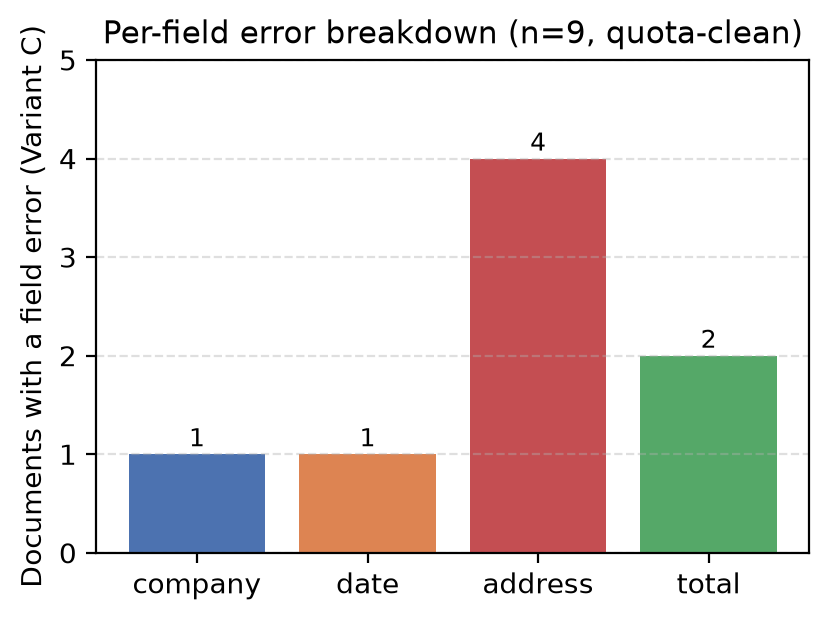
\includegraphics[width=3.0in]{fig/fig_error_by_field.png}}
    \caption{Per-field error counts for Variant C on the 9 documents. Errors concentrate in \texttt{address} (punctuation/spacing/case drift), with single errors in \texttt{company}, \texttt{date}, and two in \texttt{total} (a currency-prefix convention mismatch).}
    \label{fig:err}
\end{figure}

\subsection{Confidence Is Miscalibrated and, at This Sample Size, Non-Monotonic}
The expected calibration error of 0.204 quantifies the gap seen in the previous subsection: confidence \(0.67\) fields are correct 81.3\% of the time (above the diagonal in Fig.~\ref{fig:calib}, i.e., conservative/under-confident) while confidence \(1.0\) fields are correct only 75.0\% of the time (below the diagonal, i.e., over-confident). A well-calibrated, monotonic signal would place the higher-confidence bin at or above the lower-confidence bin's accuracy; here the ordering is inverted. With only two observed confidence levels and 9 documents, we cannot yet claim this specific inversion is a stable property of the harness rather than sampling noise; what we can claim is that raw agreement rate is not usable as a probability without calibration, and that a larger run is needed before it can be trusted to rank documents by risk. This motivates a calibration layer (e.g., temperature scaling or isotonic regression on a held-out development set) as a core component of the harness, and increasing \(N\) beyond 3 samples to obtain a finer-grained, more informative confidence signal.

\begin{figure}[htb]
\centerline{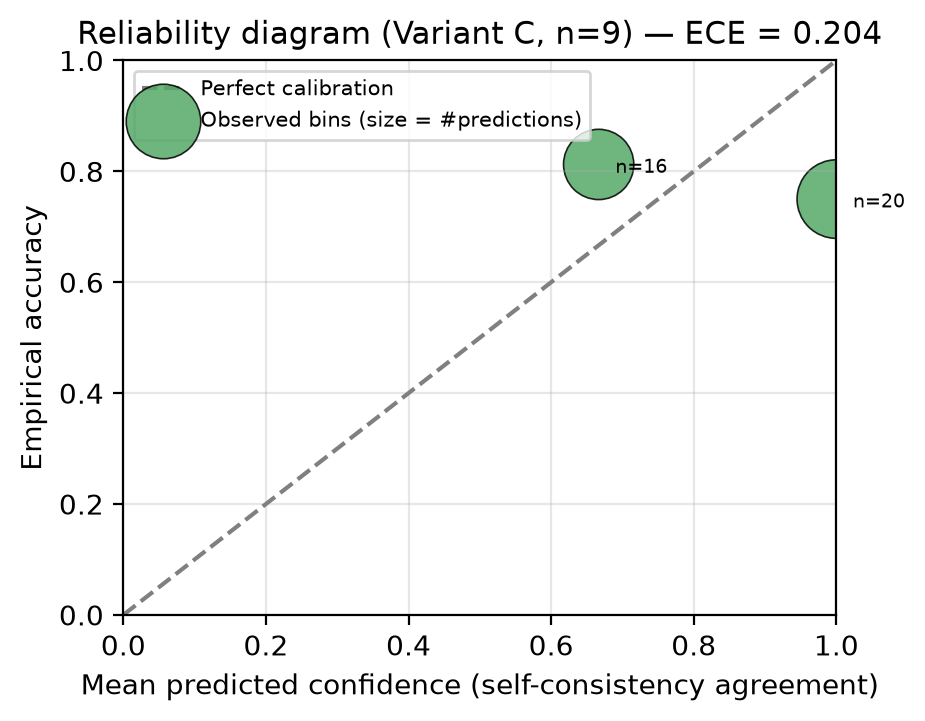
\includegraphics[width=3.0in]{fig/fig_calibration.png}}
    \caption{Reliability diagram for Variant C, \(n=9\): mean predicted confidence (self-consistency agreement) versus empirical accuracy. Marker size is proportional to the number of field predictions at that confidence level. The lower-confidence point (0.67) sits above the diagonal (conservative); the higher-confidence point (1.0) sits below it (over-confident)---an inverted ordering rather than the graded, monotonic relationship a calibrated signal should show.}
    \label{fig:calib}
\end{figure}

\subsection{Targeted Self-Correction Never Triggered in This Run}
On the 9 documents, Variant C is numerically identical to Variant B (Table~\ref{tab:results})---but not because a correction call ran and re-affirmed the majority vote. As Section~\ref{sec:confhard} established, self-consistency agreement never fell below \(\tau=0.5\) on any field in this subset, so the confidence gate never opened and \emph{zero} correction calls were issued. This is a materially weaker claim than our earlier, small-sample observation that correction ``re-affirmed values without harming them,'' and we withdraw that framing: at \(n=9\) we simply have no evidence yet, positive or negative, about what our targeted correction step does when it fires. Fig.~\ref{fig:selfcorrect} places this null result against Huang et al.\ \cite{b3}'s findings for \emph{intrinsic}, unguided self-correction (regressions of up to 34 percentage points, e.g., 75.8\%$\to$41.8\% on CommonSenseQA) and \emph{oracle-guided} correction (gains of 8--14 points): our mechanism is designed to sit in the oracle-guided regime, since it is triggered only by an external, measurable signal (self-consistency disagreement) rather than the model's own unguided judgment. The value of the mechanism as designed is that it is \emph{targeted} (only low-confidence fields), \emph{bounded} (at most one extra call per flagged field), and \emph{auditable} (the harness records which fields were flagged and corrected); its effect on accuracy when it does fire is not evidenced by this run, which reported zero flagged fields at \(\tau=0.5\).

\begin{figure}[htb]
\centerline{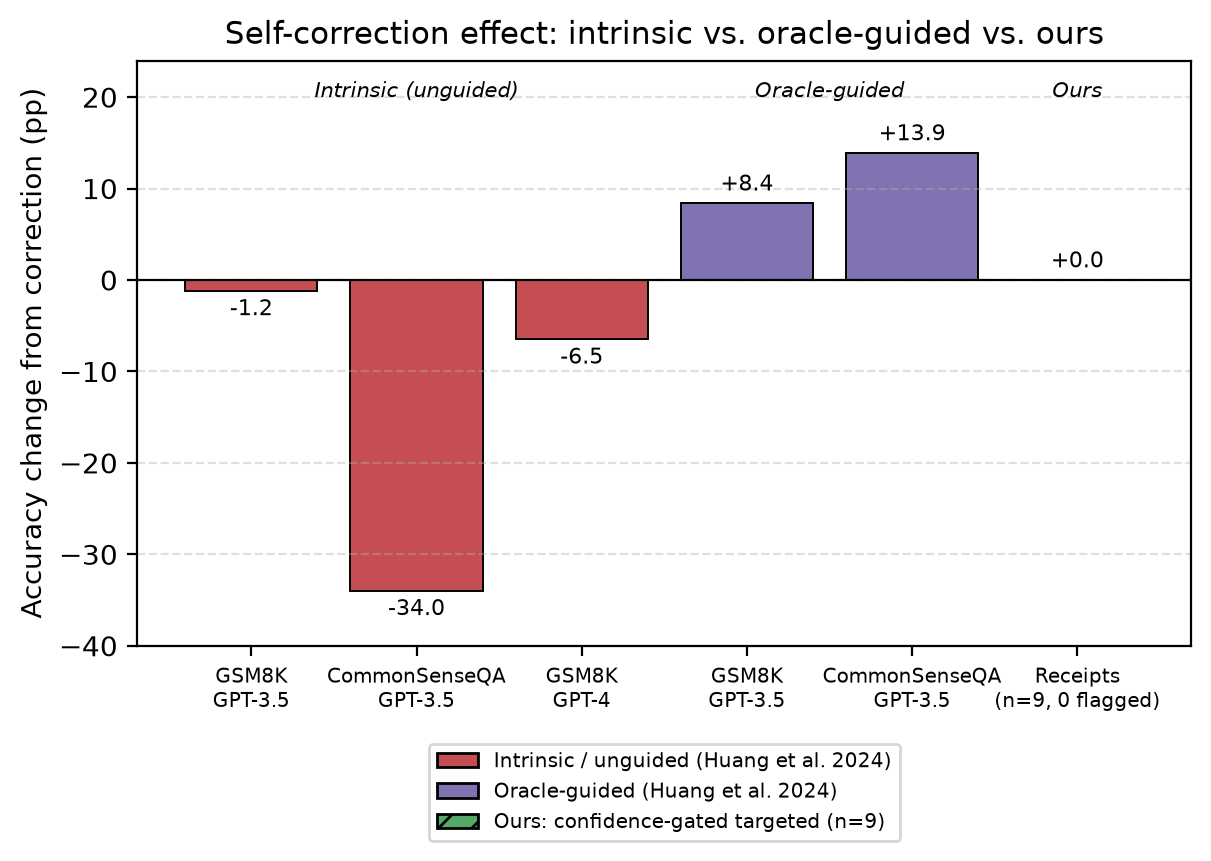
\includegraphics[width=3.4in]{fig/fig_selfcorrection_literature.png}}
    \caption{Accuracy change from a correction call: intrinsic/unguided self-correction regresses accuracy by up to 34 points, oracle-guided correction improves it by 8--14 points \cite{b3}. Our confidence-gated targeted correction shows +0.0pp because it never fired on any of the 9 documents (0 flagged), not because it fired and had no effect---this run cannot yet distinguish our mechanism from either literature regime.}
    \label{fig:selfcorrect}
\end{figure}

\subsection{Cost and Quota-Awareness}
Variant C costs at most \(N + 1\) calls per document (\(N\) samples plus up to one correction call) compared to one call for the baseline; Variant B pays a fixed \(3\times\) call budget over Variant A for the (currently indistinguishable) accuracy in Table~\ref{tab:results}. Commodity free-tier API quotas impose a strict daily ceiling on image-generation calls, and self-consistency's \(N\times\) call multiplier consumes that budget quickly, which is why the experimental harness is cache-first with retry/backoff on transient quota errors (Section~\ref{sec:expsetup})---every successful response is persisted so a run can be resumed without re-spending calls. This is itself research-relevant: it motivates a budget-aware harness that spends extra calls only when confidence is low and the document is hard, rather than always paying the full \(N\)-sample cost.

\section{Conclusion and Future Works}
\label{sec:conclusion}

This research demonstrates a harness-engineering approach to reliable document intelligence, evaluated with live model calls rather than simulation. By fixing the VLM and varying only the surrounding harness---schema, sampling policy, confidence estimator, and correction rule---we isolate and measure the contribution of each reliability mechanism on real scanned receipts. Schema-guided structured extraction provides a strong baseline (75.0\% field exact match, 97.0\% character-level F1 on 9 documents, rising to 77.8\%/98.0\% with self-consistency aggregation), consistent in order of magnitude with published SROIE and VLM-extraction results. Two findings are genuine negative/null results rather than confirmations of the design's premises: self-consistency agreement did \emph{not} reliably separate correct from incorrect extractions at this sample size, and the targeted-correction mechanism never triggered because no field's agreement fell below threshold. We view honestly reporting these limitations, rather than only the results that confirm the design's premises, as essential to the paper's reliability.

The harness perspective offers a clear path to further improvements. The modular evaluation we built is a clean reward function for harness optimization: a natural next step is to apply a Meta-Harness-style outer loop \cite{b2} that searches over prompt wording, schema descriptions, sampling counts, and confidence thresholds, using our evaluation as the reward. We also plan to:
\begin{itemize}
    \item Scale the evaluation to the full SROIE split and additional document types (forms and invoices), and report confidence intervals.
    \item Lower the confidence threshold \(\tau\) or increase \(N\) so that the correction step is actually exercised, to empirically test whether our confidence-gated correction behaves like the oracle-guided (beneficial) or intrinsic (harmful) regime in \cite{b3}.
    \item Compare self-consistency confidence against verbalized confidence and an external verifier model, and add a calibration layer on a held-out development set to correct the non-monotonicity observed in Section~\ref{sec:results}.
    \item Add a date/amount normalizer so that semantically correct near-miss extractions (e.g., the \texttt{RM}-prefix convention observed in Section~\ref{sec:results}) are not penalized by exact-match metrics.
    \item Simulate a human-review policy that routes low-confidence documents to a reviewer, quantifying the reliability gain per human intervention.
    \item Explore schema evolution: measure how extraction reliability changes as the target schema grows in size and complexity.
\end{itemize}

\begin{thebibliography}{00}
\bibitem{b1} C.~Zhou et al., ``Externalization in LLM agents: A unified review of memory, skills, protocols and harness engineering,'' arXiv preprint arXiv:2604.08224, 2026.

\bibitem{b2} Y.~Lee, R.~Nair, Q.~Zhang, K.~Lee, O.~Khattab, and C.~Finn, ``Meta-Harness: End-to-end optimization of model harnesses,'' arXiv preprint arXiv:2603.28052, 2026.

\bibitem{b3} J.~Huang et al., ``Large language models cannot self-correct reasoning yet,'' in \emph{ICLR}, 2024.

\bibitem{b4} Google AI, ``Structured outputs,'' Gemini API documentation, 2026. [Online]. Available: https://ai.google.dev/gemini-api/docs/structured-output

\bibitem{b5} X.~Wang et al., ``Self-consistency improves chain of thought reasoning in language models,'' in \emph{ICLR}, 2023.

\bibitem{b6} C.~Guo, G.~Pleiss, Y.~Sun, and K.~Weinberger, ``On calibration of modern neural networks,'' in \emph{ICML}, 2017.

\bibitem{b7} Z.~Huang et al., ``ICDAR2019 competition on scanned receipt OCR and information extraction,'' in \emph{ICDAR}, 2019.

\bibitem{b8} Y.~Xu, M.~Li, L.~Cui, S.~Huang, F.~Wei, and M.~Zhou, ``LayoutLM: Pre-training of text and layout for document image understanding,'' arXiv preprint arXiv:1912.13318, 2019.

\bibitem{b9} Y.~Xu et al., ``LayoutLMv2: Multi-modal pre-training for visually-rich document understanding,'' in \emph{ACL}, 2021.

\bibitem{b10} ``Multi-modal vision vs.\ text-based parsing: Benchmarking LLM strategies for invoice processing,'' arXiv preprint arXiv:2509.04469, 2025.

\bibitem{b11} ``Self-consistency boosts calibration for math reasoning,'' arXiv preprint arXiv:2403.09849, 2024.

\end{thebibliography}

\end{document}
